\documentclass[a4paper,oneside]{bth}

\usepackage{amsmath}
\usepackage{mathenv}
\usepackage{amssymb}
\usepackage{amsthm}
\usepackage{textcomp}
\usepackage{longtable}
\usepackage{multirow}
\usepackage{pifont}
\usepackage{changepage}
\usepackage{listings}
\usepackage{url}
\usepackage{xspace}
\usepackage{xtab}
\usepackage[utf8]{inputenc}
\usepackage[T1]{fontenc}
\usepackage{graphicx}
\usepackage{enumitem}
\usepackage{dirtytalk}
\usepackage{wrapfig}
\usepackage{float}
\usepackage[section]{placeins}
\usepackage[export]{adjustbox}
\usepackage{caption}
\usepackage{subcaption}
\DeclareGraphicsExtensions{.pdf}

\newtheorem{lem}{\textsc{Lemma}}[chapter]
\newtheorem{thm}{\textsc{Theorem}}[chapter]
\newtheorem{prop}{\textsc{Proposition}}[chapter]
\newtheorem{post}{Postulate}[chapter]
\newtheorem{corr}{\textsc{Corollary}}[chapter]
\newtheorem{defs}{\textsc{Definition}}[chapter]
\newtheorem{cons}{\textsc{Constraint}}[chapter]
\newtheorem{ex}{\textbf{Example}}[chapter]
\newtheorem{qu}{\textbf{Question}}[chapter]

\begin{document}
\pagestyle{plain}
\pagenumbering{gobble}
\setlength{\parindent}{0em}

%%%%%%%%%%%%%%%%%%%%%%%%%%%%%%%%%%%%%%%%%%%%%%%%%%%%%
% Front matter

{
\pagestyle{empty}
\changepage{5cm}{1cm}{-0.5cm}{-0.5cm}{}{-2cm}{}{}{}
\noindent%
{\small
\begin{tabular}{p{0.75\textwidth} p{0.25\textwidth}}
\textit{Bachelor Thesis}&\multirow{4}{*}{\bthcsnotextlogo{3cm}}\\
\textit{Software Engineering}\\
\textit{urn:nbn:se:bth-14888}\\
\textit{06-2017}\\
\end{tabular}}

\begin{center}

\par\vspace {7cm}

{\Huge\textbf{Performance characteristics between monolithic and microservice-based systems\\*[1cm]}}  

\par\vspace {0.5cm}

%{\Large\textbf{Centered Subtitle Times Font Size 16 Bold}}                   

\par\vspace {3cm}

{\Large\textbf{Robin Flygare}}
\par\vspace {0.3cm}
{\Large\textbf{Anthon Holmqvist}}
\par\vspace {4cm}

\end{center}

\noindent%

{\small Faculty of Computing\\
Blekinge Institute of Technology\\
SE--371 79 Karlskrona, Sweden}
}

%%%%%%%%%%%%%%%%%%%%%%%%%%%%%%%%%%%%%%%%%%%%%%%%%%%%%

\clearpage

{\pagestyle{empty}
\changepage{5cm}{1cm}{-0.5cm}{-0.5cm}{}{-2cm}{}{}{}
\noindent
\begin{tabular}{p{\textwidth}}
{\small This thesis is submitted to the Faculty of Computing at Blekinge Institute of Technology in partial fulfillment of the requirements for the degree of Bachelor of Science in Software Engineering. The thesis is equivalent to 10 weeks of full time studies.}
\end{tabular}

\par\vspace {12cm}

\noindent%
\begin{tabular}{p{0.5\textwidth}lcl}
\textbf{Contact information}\\
Authors:\\
Robin Flygare\\
Email: robin.flygare1@gmail.com\\
Anthon Holmquist\\
Email: anthon.kendel@gmail.com\\

\par\vspace {4cm}
University advisor:\\
Dr. Richard Berntsson Svensson\\
Department of Software Engineering\\

\par\vspace {1cm}
\noindent%
 \\

Dept. Computer Science \& Engineering & Internet & : & www.bth.se/didd\\
Blekinge Institute of Technology & Phone	& : & +46 455 38 50 00 \\
SE--371 79 Karlskrona, Sweden & Fax & : & +46 455 38 50 57 \\

\end{tabular}
\clearpage
} % Back to \pagestyle{plain}

\setcounter{page}{1}

% ABSTRACT

\abstract
\begin{changemargin}{+1cm}{+1cm}
\noindent

%%1-2 sentence area of concern
\par\vspace {0.5cm}
A new promising technology to face the problem of scalability and availability is the microservice architecture. The problem with this architecture is that there is no significant study that clearly proves the performance differences compared to the monolithic architecture.

%1 sentence problem
\par\vspace {0.5cm}
Our thesis aims to provide a more conclusive answer of how the microservice architecture differs performance wise compared to the monolithic architecture.

%1-2 method and data collection
\par\vspace {0.5cm}
In this study, we conducted several experiments on a self-developed microservice and monolithic system. We used JMeter to simulate users and after running the tests we looked at the latency, successful throughput for the tests and measured the RAM and CPU usage with Datadog.

%2-3 sentence data analysis
\par\vspace {0.5cm}
Results that were found, were that the microservice architecture can be more beneficial than the monolithic architecture. Docker was also proven to not have any negative impact on performance and computer cluster can improve performance.

%1-2 sentence conclusion and contribution
\par\vspace {0.5cm}
We have presented a conclusive answer that microservices can be better in some cases than a monolithic architecture.
\par\vspace {1cm}
% 3-4 keywords, maximum 2 of these from the title, starts 1 line below the
% abstract.
\noindent\\
\textbf{Keywords:} Performance, Microservices, Docker, Container

\end{changemargin}

\include{acknowledgments} %OPTIONAL

\section*{Acknowledgements}
We would first like to thank our university advisor Dr. Richard Berntsson Svensson of the Department of Software Engineering at Blekinge Institute of Technology. The door to Dr. Richard Berntssson Svensson office was always open whenever we ran into a troubled spot or had a question about our research or writing. He consistently allowed this paper to be our own work, but steered us in the right the direction whenever he thought we needed it.

\par\vspace{0.5cm}
We would also like to thank Ruwan Lakmal Silva and Pär Karlsson of Ericsson, Karlskrona for the suggestions for a thesis. We are grateful for their valuable comments and guiding us on the right path.
%\listoffigures %in case you have them
%\listoftables %in case you have them
%\listofalgorithms %in case you have them
\tableofcontents 

\cleardoublepage
\pagestyle{headings}
\pagenumbering{arabic}

\chapter{Introduction}

%STARTS WITH background to the general area (area of concern) and ends with problem
As the world keeps expanding more and more people are gaining access to computers and the internet. This put demands on systems that they always should be available and reliable \cite{Bondi}. From this problem of demand, more and more software companies have started to research new architectures that should solve these problems \cite{farrow-netflix}.

\par\vspace {0.5cm}
Currently, a new promising architecture for these traits is the microservice architecture \cite{Fowler}. Since the microservice architecture is a new concept, there is still the question about how much really the architecture affects the performance compared to a monolithic architecture, there are studies that show performance differences ranging from a performance increase to a 79.2\% decrease in performance when using containers \cite{Joy, Ueda}.

\par\vspace {0.5cm}
%STARTS WITH what we need to analyze the problem or gap
To analyze the performance differences, we need to study the available research in performance comparison. Since there are many architectures which can be classified as a microservice architecture we need to provide a minimal working architecture for both microservices and monolithic. We then need to look at the performance and compare it to the related research to get a better view of how and why the performance differs.

\par\vspace {0.5cm}
%STARTS WITH method research process to study problem. describes how data collection will be done and ends with how data analysis will be done
In our thesis we conducted several experiments with microservices and monolithic architectures, we then analyze these to conclude our thesis. In our experiment, we will collect RAM and CPU usage using Datadog and successful throughput, latency, error rate will be collected with JMeter. All data is manually analyzed to find out where the different architectures differ in performance.

\par\vspace {0.5cm}
%Describes which types of contributions the paper will make. if short paragraph add it to 3rd paragraph instead
Our research aims to provide a more conclusive answer of how the microservice architecture performs compared to the monolithic architecture. 
Our goals for this thesis are:

\begin{enumerate}

\item To provide data, result, and conclusions, of the performance differences between monolithic and microservice systems.
\item To know when it is beneficial to use monolithic systems over microservices systems.
\item To know when it is beneficial to use microservices systems over monolithic systems. 
\item To understand the performance differences between a single machine microservice versus a computer cluster microservice.
    
\end{enumerate}

\par\vspace {0.5cm}
%Outline of the paper, text based version of a table of content that only outlines what your main sections (header level 1)will bring up.
This thesis starts with presenting our research questions in Chapter \ref{RQ}. In Chapter \ref{relatedWork} we write about and summarize related research done in the area. In Chapter \ref{Method} we explain our method. In Chapter \ref{Results} we present our results. In Chapter \ref{Analysis} we present an analyze of the results and in Chapter \ref{Conclusion} we conclude the thesis with a conclusion. From this, we summarize existing research and see if there is already an answer on any of our research questions. We then present our result from our experiment where this follows by a conclusion and future work about what we believe to be left to be done.

%%%%%%%%%%%%%%%%%%%%%%%%%%%%%%%%%%%%%%%%%%%%%%%%%%%%%

\chapter{Research questions} \label{RQ}

The definition of what performance characteristics we are measuring can be found in chapter \ref{relatedWork}.\\

\textbf{RQ1. What is the performance difference between a monolithic system versus a microservice-based system?}\\
The purpose of this question is to provide performance data and research that will be used to determine when and where it is better to use one system over the other. The data and results will be used as a basis for the analysis and conclusions between the system. Answering this question will provide a good base of knowledge for future work and research in the area of microservices and monolithic systems.

\par\vspace {0.5cm}
\textbf{RQ2. What is the performance difference when running a monolithic system in Docker vs bare-metal?}\\
The purpose of this question is to provide performance data and research that will be used to determine the general performance overhead in containers. The data and results will be used as a basis for the analysis and conclusion of what areas are affected and how these areas differ between the systems. Answering this question will provide information and results of what the impacts and which areas are affected when using Docker for microservices and monolithic systems.

\par\vspace {0.5cm}
\textbf{RQ3. What is the performance difference when running a microservice-based system on one machine versus a computer cluster?}\\
The purpose of this question is to provide information and data on the performance differences between a single machine microservice versus a computer cluster microservice. The data and result will be used as a basis for the analysis and conclusion of when a cluster or a single machine is more beneficial.

%%%%%%%%%%%%%%%%%%%%%%%%%%%%%%%%%%%%%%%%%%%%%%%%%%%%%

\chapter{Related work} \label{relatedWork}

Fowler presents the differences between a monolithic architecture and a microservice architecture \cite{Fowler}. To understand what our research is about it is crucial to understand the differences between these architectures. In Fowler’s article, he explains the microservice architecture as a suite of small services. Each one of these services is running its own process and communicates with the other services with a lightweight interface such as an HTTP API. Fowler continues to explain the monolithic architecture as a single unit, were enterprise applications usually are built in three parts: a client user interface, a server-side application, and a database. A monolithic system consists of a single logical executable, the server side application. In Fowler’s article, he continues to explain the differences between a microservice architecture and a monolithic architecture, the most important differences are:

\begin{enumerate}

\item A microservices architecture has several processes while a monolithic architecture only has one process.
\item A microservice can be developed independently from other microservices while a monolithic architecture is developed as a single application with classes, functions, and namespaces.
\item A microservice can scale independently from other microservices while in the monolithic architecture the whole application must scale.
\item A microservice can be changed and be deployed without deploying other microservices while in the monolithic architecture the whole application needs to be deployed.

\end{enumerate}

Continuing Fowler's article about microservices, existing research investigates why the microservice architecture has not been used, where Xavier et al. writes about how traditionally virtualization technologies have been avoided due to the performance overhead, but with the rise of container-based (microservices) implementations it is now possible to obtain a very low overhead leading to near native performance \cite{Xavier}. G. Xavier et al. conducted several experiments to evaluate the performance in containers compared to Xen. Xen is a hypervisor system for virtual machines. Their study concluded that containers provide near-native performance, but have bad isolation in memory, disk, and network.

\par\vspace {0.5cm}

Research also investigates the problems and impact of breaking a monolithic application into several microservices. Knoche writes about breaking up a monolithic system requires careful planning and may have a severe impact on the performance \cite{Knoche}. Knoche presents an eight-step incremental approach for sustaining performance when breaking down a monolithic system into microservices. The approach includes performance simulation for seeing what the expected performance is when the microservice-based architecture is used. Knoche presents different paths for implementing the modern microservice-based architecture. Each path performance results from the simulations are presented where the developer can decide on a path for their implementation of the microservice-based architecture.

\par\vspace {0.5cm}

Furthermore, Balalaie et al. present experiences and lessons learned when incrementally migrating from a service to a microservice architecture \cite{Balalaie}. They write about how they were moving from a monolithic pipeline to microservices pipeline which is independent for each service, so they can be deployed independently. Moving from monolithic to microservices presents an option of multiple cross-functional teams which enable DevOps.

\par\vspace {0.5cm}

Continuing the positive trend on moving from monolithic systems to microservices, we have found that in existing research there is a big focus on figuring out how the system will be affected when moving from a monolithic architecture to a microservice architecture. Ueda et al. write about the performance impact when using Node.js or Java as the main application, Docker for isolating the different parts of the applications to implement the microservice architecture, MongoDB for database and Apache JMeter for their performance tests \cite{Ueda}. The study measured bare-process, with Docker host and with Docker bridge. They found that with these parameters microservices implementations had worse performance than their monolithic counterparts, up to 79.2\% in Node.js and 70.2\% in Java.

\par\vspace {0.5cm}

Villamizar et al. compared the average response time between a monolithic and a microservice-based system in the cloud. In their test, both systems were deployed to Amazon Web Services with similar hardware \cite{Villamizar}. Villamizar et al. describe their test results as that there is a minimal performance impact and that both systems would fulfil the case study requirements where they had two services, S1 and S2. The case study requirements were defined as: \say{The service S1 implements CPU intensive algorithms to generate every payment plan and their typical response time is around 3000 milliseconds.} and \say{The typical response time of service S2 is around 300 milliseconds and this service consumes mainly the database.}. Villamizar et al. furthermore explain that hosting their solution would be 17\% cheaper for the microservice architecture on Amazon Web Services.

\par\vspace {0.5cm}

There are also different ways to use a microservice architecture which may provide different performance results, Amaral et al. compared the performance differences in throughput and latency of two different microservice architectures, master-slave, and nested containers \cite{Amaral}. The master-slave architecture is explained as it is composed of one container as the master container which is coordinating the other containers which are called slaves. The nested container architecture is that the containers are hierarchically created into the main container. They found that the when using virtual machines the latency is approximately 12\% higher. They concluded that nested containers are a suitable microservice architecture as an addition to the regular master-slave container architecture. When running the performance benchmark Sysbench, with increasing the number of instances relative to a single Sysbench instance in bare-metal, they found no significant performance impact for CPU-intensive executions on containers or virtual machines compared to bare-metal. This is because containers are only isolated by a lightweight layer and virtual machines have gotten much better with virtualization support in modern processors.

\par\vspace {0.5cm}

There are also other studies comparing the performance of bare-metal, virtual machines, and containers. Kalidindi writes about how running Cassandra in containers would provide a performance gain compared to virtual machines \cite{Kalidindi}. Kalidindi presents an implementation model of a Cassandra cluster based on realistic scenarios, and then measure the difference between bare-metal and using Docker. Kalidindi found that disk utilization in both bare-metal and Docker showed equivalent values when under mixed load with bare-metal slightly outperforming. The study showed that when using containers there was a slight latency overhead of 6-8\% in read and write. Vangeepuram instead writes about the performance difference in Cassandra when running bare-metal compared to with containers, for different load scenarios \cite{Vangeepuram}. The comparison is done on CPU utilization and disk throughput. Vangeepuram observed overhead when running containers, higher CPU usage and higher disk throughput except in one scenario. The study also presents that Cassandra has lower latency in all scenarios when running bare-metal. 

\par\vspace {0.5cm}

As we have seen a positive trend with migrating monolithic applications to microservices, the demand on the system presents the need to run multiple instances of an application. \say{A distributed application is software that is executed or runs on multiple computers within a network}, explained by Technopedia \cite{Technopedia}. The differences between traditional and distributed applications are that instead of relying on a single system to run the application, distributed application runs the application on multiple systems, so if a system goes down, the other system can resume the task.

\par\vspace {0.5cm}

Joy writes about how modern distributed applications are running on virtualized environments for benefits in hardware utilization and flexibility in the infrastructure \cite{Joy}. Containers can provide an alternative to the traditional virtualization and therefore increase utilization and reduce the overhead that virtualization provides. In the study, Joy compares the performance and scalability of containers and virtual machines. The study showed that containers could handle more requests and had better scalability than virtual machines.

\par\vspace {0.5cm}

From our literature study, we found results that present that containers have none or very little performance deficit compared to running on physical hardware. We also found results from studies that shows that there are major differences of up to 79.2\% worse performance between monolithic and microservices systems. In all studies regarding microservices versus virtual machines, we found out that microservices are better than a traditional virtual machine. We conclude that this suggests that there is no clear picture of the real performance impact of microservices compared to monolithic systems. We have seen that the performance will be dependent on several different factors such as programming language, environment, database technology, container technology and system architecture.

\par\vspace {0.5cm}
In the related work, there was no conclusive answer found of the performance differences, therefore it is important to study this which is the focus of this thesis.

%%%%%%%%%%%%%%%%%%%%%%%%%%%%%%%%%%%%%%%%%%%%%%%%%%%%%

\chapter{Method} \label{Method}

For our method we chose to conduct an experiment \cite{Juristo:2010:BSE:1965114}. We chose to conduct an experiment because we wanted to see actual numbers of the performance differences which we could not get from a case study, interview or a questionnaire. Furthermore, we chose this since we wanted to see the performance differences between the architectures related to microservices and monoliths, more specifically A1, A2, A3, and A4. The legend and definitions for these architectures can be found in figures \ref{fig:Legend}, \ref{fig:A1}, \ref{fig:A2}, \ref{fig:A3} and \ref{fig:A4}.

\par\vspace {0.5cm}

For our experiment, we developed an application and collected performance data.  Performance aspects were RAM usage, CPU usage, latency, error rate and successful throughput. The application is developed in two versions: one monolithic version, and one microservices version. Both versions use a minimal architecture in both cases. The application was tested against a set of defined stress tests and performance data was collected. We deployed our application to one machine and several machines to simulate both a single server and a computer cluster.


\section{Experiment design} \label{experimentDesign}

The Experiment design starts with the Experiment definition which explains why chose to conduct the experiment and continues with an explanation of the architectures and setting. After this, we present the Independent variables and Dependent variables. This follows with our hypothesis and what we think the experiment will result in. Our Experiment design ends with how we did the experiment and what tools we used to collect our performance data.

\subsection{Experiment definition}

As presented in Related work there are several papers \cite{Villamizar, Amaral, Kalidindi} conducting experiments regarding monolithic architectures versus microservice architectures. These papers present different aspect of performance and the results differ from each other. Therefore, we felt the need to explore this area further, therefore we chose to conduct an experiment because we wanted to see actual numbers of the performance differences and compare our results with other papers. In our experiment, we present our hypothesis regarding our research questions and in Chapter 5 and Chapter 6 we present our actual result and conclusions.

\subsection{Research setting} \label{researchSetting}

Our research setting will simulate a complete system which includes user interface, REST API, business logic and a database. In the following sections, we will explain the different functions and services in this system.

\par\vspace {0.5cm}
The primary key is automatically generated in Scala \cite{Scala} using the UUID Java class \cite{uuid} and is not counted as a property for our test cases found in section \ref{measurementObjects}. To get a more realistic example of the microservice architecture, we will encrypt the data using SHA-256 \cite{SHA} and 16 bytes AES \cite{AES}. The data will then be saved into Cassandra \cite{Cassandra}, our chosen system storage technology.

\par\vspace {0.5cm}
We use slightly modified Akka-HTTP settings in our configuration.
We use eight max connections and 1024 max open requests so the requests do not get rejected as much by Akka because of the load testing.

\par\vspace {0.5cm}
When communicating between containers in the A1 microservice architecture we choose to use the built-in Docker bridge feature. This gives us the ability to evaluate the network latency difference correctly because when running as Docker host the containers’ networks are not isolated from the host system. In the A2 cluster microservice architecture we use the host system since the computers need to communicate and we chose not to use an orchestration software for this.

\begin{wrapfigure}{r}{0.4\textwidth}
\begin{center}

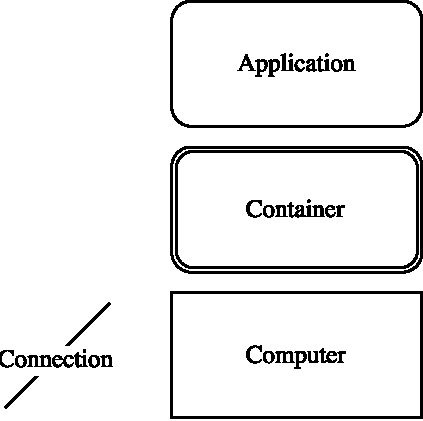
\includegraphics[width=0.3\textwidth]{Legend}
\caption{Legend explaining the different concepts}
\label{fig:Legend}

\end{center}
\end{wrapfigure}

\par\vspace {0.5cm}
Following hardware was used for our experiment: 2x Intel NUC5i7RYH with the following specifications: 16GB RAM, Intel Core i7-5557U Processor, and Ubuntu Server 16.04 as host operating system.
For our tests, JMeter was executed from a computer on the same local network as the other machines, running Windows 10 pro with an Intel Core i54690K processor and 16GB RAM.

\clearpage
We evaluated our experiment on four architectures A1, A2, A3, and A4, the legend explanation for these architectures can be seen in figure \ref{fig:Legend}. 

\begin{enumerate}[label=A\arabic*]

\item The microservice architecture on one machine. Shown in figure \ref{fig:A1}.
\item The microservice architecture split into two machines. Shown in figure \ref{fig:A2}.
\item The monolithic architecture running inside a container on one machine. Shown in figure \ref{fig:A3}.
\item The monolithic architecture running directly on one machine. (bare-metal) Shown in figure \ref{fig:A4}.

\end{enumerate}

\textbf{Microservices}

The microservice-based architecture is split into four microservices, each running in its own Docker container.

\par\vspace {0.5cm}
For the user interface, we used HTML5, CSS3 and jQuery 3.2.0. For the REST interface we used Scala 2.11.8, Java 8 with JDK 1.8.0, SBT 0.13.15 and Akka HTTP 10.0.5.

\par\vspace {0.5cm}
For the microservices running services and communicating with the REST interface and Cassandra we used Scala 2.11.8, Java 8 with JDK 1.8.0, SBT 0.13.15, Akka HTTP 10.0.5, Spark Cassandra Connector 2.0 and Spark 2.1. As for our database service, we used Cassandra 3.0.

\begin{figure}[h]
\begin{center}

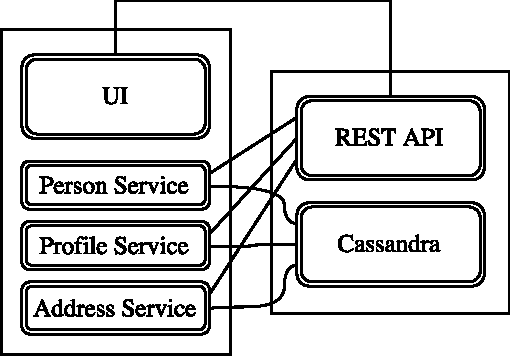
\includegraphics[width=0.31\textwidth]{A2/A2}
\caption{Microservice architecture split onto two machines}
\label{fig:A2}

\end{center}
\end{figure}

\begin{figure}[H]
\begin{center}

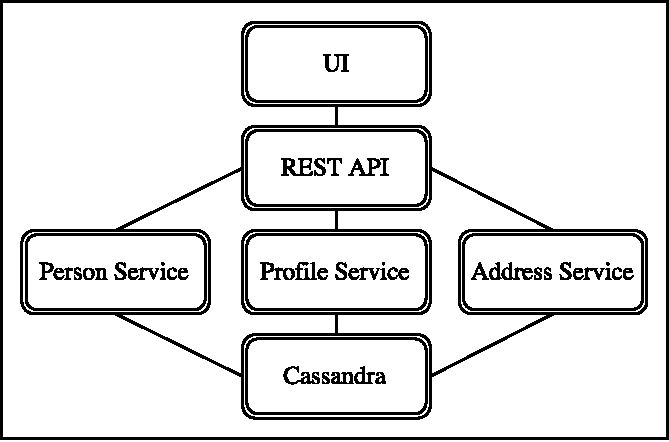
\includegraphics[width=0.35\textwidth]{A1/A1}
\caption{Microservice architecture on one machine}
\label{fig:A1}

\end{center}
\end{figure}

%%%%%%%%%%%%%%%%%%%%%%%%%%%%%%%%%%%%%%%%%%%%%%%%%%%%%

\clearpage
\par\vspace {0.5cm}

\textbf{Monolithic}

The monolithic system is split into three parts.

\par\vspace {0.5cm}
For the user interface we used HTML5, CSS3 and jQuery 3.2.0. For the application we used Scala 2.11.8, Java 8 with JDK 1.8.0, SBT 0.13.15 and Akka HTTP 10.0.5, Spark Cassandra Connector 2.0 and Spark 2.1. As for our database, we used an instance of Cassandra 3.0.

\begin{figure}[h]
\begin{center}

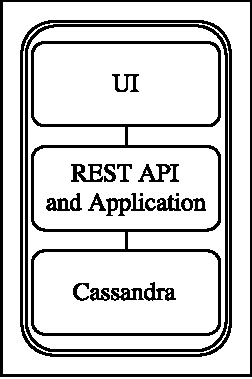
\includegraphics[width=0.2\textwidth]{A3/A3}
\caption{Monolithic architecture running inside a container on one machine.}
\label{fig:A3}

\end{center}
\end{figure}

\begin{figure}[h]
\begin{center}

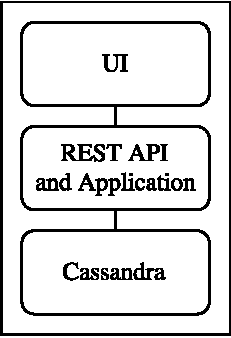
\includegraphics[width=0.2\textwidth]{A4/A4}
\caption{Monolithic architecture running directly on one machine. (bare-metal)}
\label{fig:A4}

\end{center}
\end{figure}

%%%%%%%%%%%%%%%%%%%%%%%%%%%%%%%%%%%%%%%%%%%%%%%%%%%%%

\clearpage
\par\vspace {0.5cm}

\subsection{Independent variables}
The independent variables for our experiment is the number of users simulated by JMeter and the architectures explained in section \ref{researchSetting}.
Another independent variable is containerizing the system using Docker.
\subsection{Dependent variables}
The dependent variables for our experiment is the RAM usage, CPU usage, latency, error rate and successful throughput.

\subsection{Hypothesis}
Our hypothesis for our experiment is the following:

\begin{enumerate}[label=RQ\arabic*]

\item The A4 bare-metal monolithic architecture will have lower CPU usage, lower RAM usage, lower latency, and higher successful throughput compared to the A1 microservice architecture.

\item  The A4 bare-metal monolithic architecture will have lower CPU usage, lower RAM usage, lower latency, and higher successful throughput compared to the A3 containerized monolithic architecture.

\item The A2 cluster architecture will have higher CPU usage, higher RAM usage, higher latency and higher successful throughput compared to the A1 microservice architecture.

\end{enumerate}

\subsection{Experimental steps}

Our experiment was divided into two parts: development of an application and executing it against test cases defined in section \ref{measurementObjects} and collecting of performance data.

\subsection{Measurement instruments}

For our measurements in CPU and RAM usage, we used Datadog \cite{Datadog}. We installed the Datadog agent on both Intel NUC computers, where the agent sent the data to Datadog, where we later analyzed the data. We used JMeter 3.2 \cite{JMeter} for simulating usage and measuring response time, error rate and
successful throughput.

\subsection{Measurement objects} \label{measurementObjects}

All our measurements are done in a test plan for JMeter. In our test plan, we use a ramp up period of 60 seconds and run each test case for two minutes following with  a delay of two minutes before starting the next. Note that in our test cases JMeter acts as users interacting with the user interface and makes REST request.

A property can be for example a first name, last name or a phone number.

\begin{enumerate}[label=TC\arabic*]

\item Create a Person and fetch a Person (2 properties)
\begin{enumerate}

\item 1 simultaneous user
\item 10 simultaneous users
\item 100 simultaneous users
\item 1000 simultaneous users

\end{enumerate}

\item Create an Address and fetch an Address (5 properties)
\begin{enumerate}

\item 1 simultaneous user
\item 10 simultaneous users
\item 100 simultaneous users
\item 1000 simultaneous users

\end{enumerate}

\item Create a Profile and fetch a Profile (10 properties)
\begin{enumerate}

\item 1 simultaneous user
\item 10 simultaneous users
\item 100 simultaneous users
\item 1000 simultaneous users

\end{enumerate}

\item All of the above test cases concurrently
\begin{enumerate}

\item 1 simultaneous user
\item 10 simultaneous users
\item 100 simultaneous users
\item 1000 simultaneous users

\end{enumerate}

\end{enumerate}

\section{Data collection}
For the experiment, we prepared our computers with all dependencies to be able to run our applications. Before running our test plan in JMeter we made sure that no unnecessary services or background tasks were running that could interfere with impact on the performance. After this, we started all containers and services that were necessary to run a specific architecture where we did this in numerical order from A1 to A4. When a test plan was completed we took snapshots of CPU usage and RAM usage on the executed architecture.

\par\vspace{0.5cm}
Latency, successful throughput and error rate was collected from JMeter in CSV files.
\section{Data analysis}

With the help of JMeter, all our data was saved into CSV files which were imported into Excel where we analyzed the data and summarized it into diagrams and tables.

\par\vspace{0.5cm}
All data was collected with tools built into JMeter, the performance aspects collected from JMeter was average response time, 90\%-line response time, error rate and throughput. All these aspects helped us understand what happened and which architecture was affected when increasing the number of users. One thing to note is that we will only use the aspects that will help to answer our research questions. 

\par\vspace{0.5cm}
When analyzing the collected data we focused on answering our research questions. We used both diagrams and numbers to find the differences between the different architectures. Our result from our experiment is presented in Results and Analysis.

\section{Validity threats}
%ANNOUNCEING MOVE, identifying limitations and explaning how important they are.
%REFLECTING MOVE, Explaining the nature of the limitations and justifying the choices you made
%FORWARDLOOKING MOVE, Suggesting how such limitations could be overcome in future
One of the validity threats \cite{Juristo:2010:BSE:1965114} are that we have a rather small amount of users tested. With more users, we think a better picture of scalability could have been seen. The reason we chose to not include more test cases was that we had to modify settings in the tools and that they were not able to handle all requests at 1000 users even. To overcome this limitation it is possible to create more test cases with better hardware, which in our case was not accessible or possible with the resources we had available. 

\par\vspace{0.5cm}
Another validity threat was a bug in the spark version we used \cite{SparkBug}. This made some of the requests return an error. The reason we used this version was because it was the latest officially supported version. To overcome this error you can update to Spark version 2.2 when released.

%%%%%%%%%%%%%%%%%%%%%%%%%%%%%%%%%%%%%%%%%%%%%%%%%%%%%

\chapter{Results} \label{Results}

\section{Monolithic architecture versus microservice architecture (RQ1)}
%SHORT SUMMARY OF RQ AND THEN FOLLOW UP WITH EVERYTHING RELATED TO RQ
RQ1 aims to provide an answer about the performance difference when running an application in the A1 microservice architecture compared to the A4 monolithic bare-metal architecture.

\par\vspace{0.5cm}
When running our tests on the A1 microservice architecture we found that the average CPU usage was 46.65\% and the total memory usage was 13.42 GiB. When running our tests on the A4 monolithic architecture we found that the average CPU usage was 49.12\% and the total memory usage was 8.07 GiB. 

\par\vspace{0.5cm}
This means that we saw an increase of 2.47 percentage points in CPU usage in the monolithic architecture using 5.36 GiB less RAM compared to the microservices architecture.

\par\vspace{0.5cm}
In figure \ref{rq1-latency}a and \ref{rq1-latency}b  we can observe the difference in latency for A1 and A4. In this result we can see that A4 has lower latency in all test cases except when there is 1000 users, why this result is explained in our Analysis. For one user, we see that A1 is 14\% slower, for 10 users we can see that A1 is 12\% slower, for 100 users A1 is 31\% slower, and lastly for 1000 users A1 is 130\% faster. 

\par\vspace{0.5cm}
Furthermore, we can see the throughput of successfully request in figure \ref{rq1-stps}. In this figure, we can see that A4 has higher throughput rate in all test cases compared to A1. For one user, we can see that A1 has 14\% lower successful throughput, for 10 users it has 4\% lower, for 100 users it has 5\% lower and for 1000 users it has 19\% lower successful throughput.
In figure \ref{rq1-error} we can see the error rate for the A1 and A4 architectures, we later use this in the chapter Analysis to explain the differences in a few of the test cases.

\begin{figure}[h]
\begin{center}

\begin{subfigure}[b]{1\textwidth}
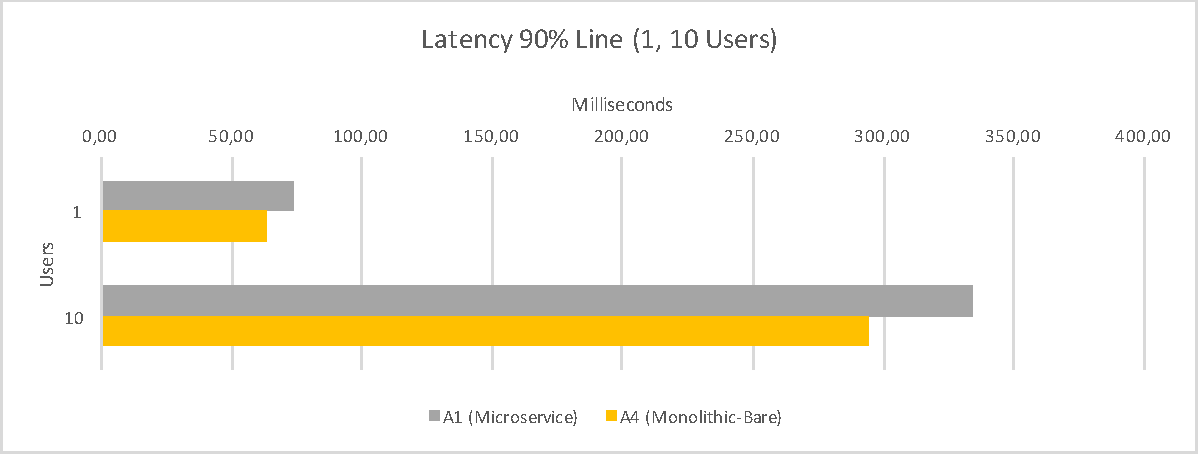
\includegraphics[width=13cm]{Graph/rq1-latency-1}
\caption{Comparison of the latency in A1 and A4 for 1 and 10 users}
\end{subfigure}

\begin{subfigure}[b]{1\textwidth}
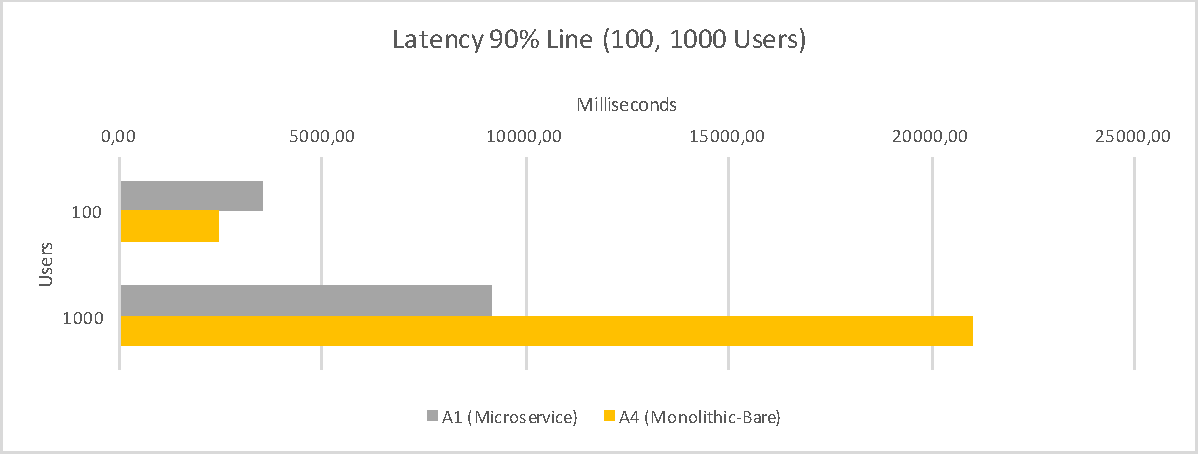
\includegraphics[width=13cm]{Graph/rq1-latency-2}
\caption{Comparison of the latency in A1 and A4 for 100 and 1000 users}
\end{subfigure}

\caption{Comparison of the latency in A1 and A4}
\label{rq1-latency}

\end{center}
\end{figure}


\begin{figure}[h]
\begin{center}

\begin{subfigure}[b]{1\textwidth}
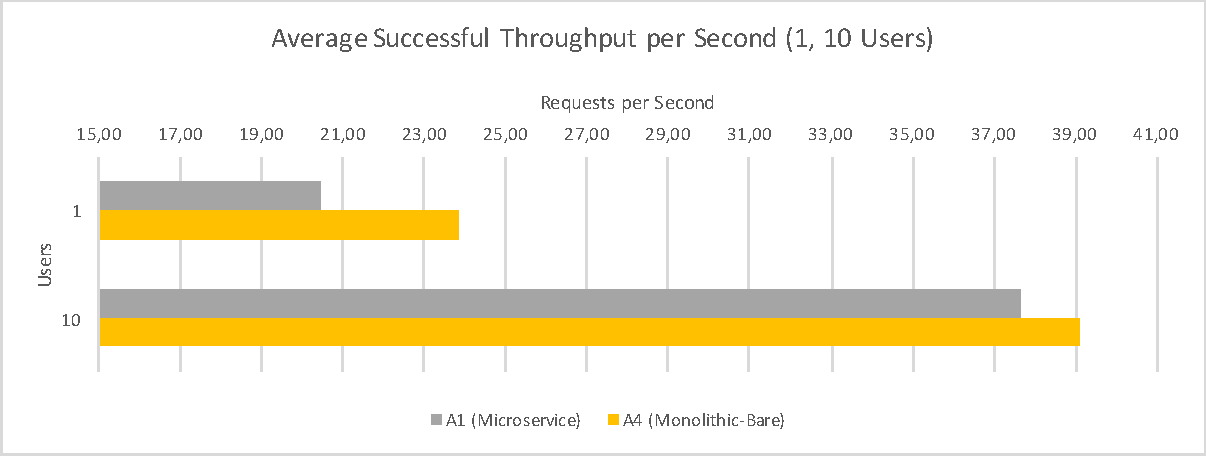
\includegraphics[width=13cm]{Graph/rq1-stps-1}
\caption{Comparison of the successful throughput in A1 and A4 for 1 and 10 users}
\end{subfigure}

\begin{subfigure}[b]{1\textwidth}
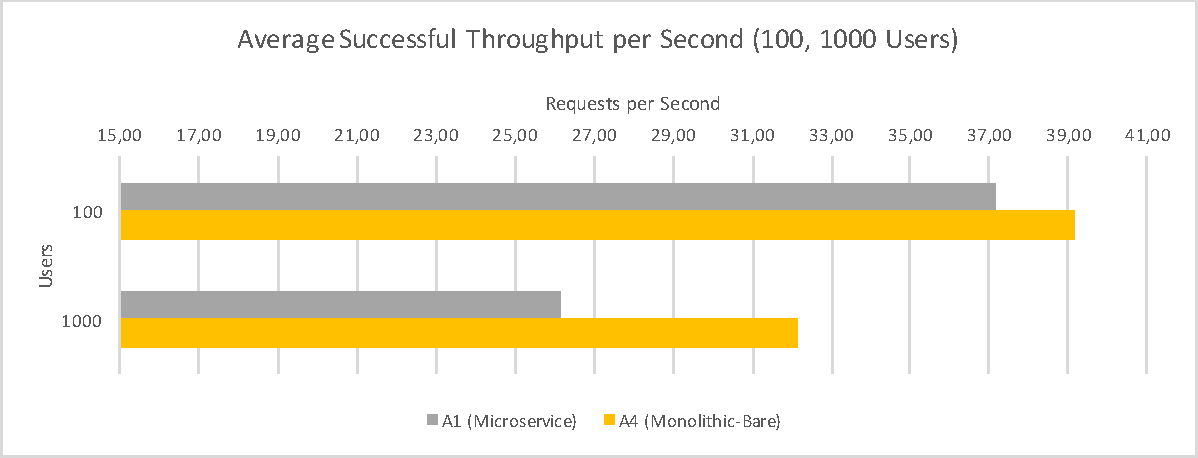
\includegraphics[width=13cm]{Graph/rq1-stps-2}
\caption{Comparison of the successful throughput in A1 and A4 for 100 and 1000 users}
\end{subfigure}

\caption{Comparison of the successful throughput in A1 and A4}
\label{rq1-stps}

\end{center}
\end{figure}

\begin{figure}[h]
\begin{center}
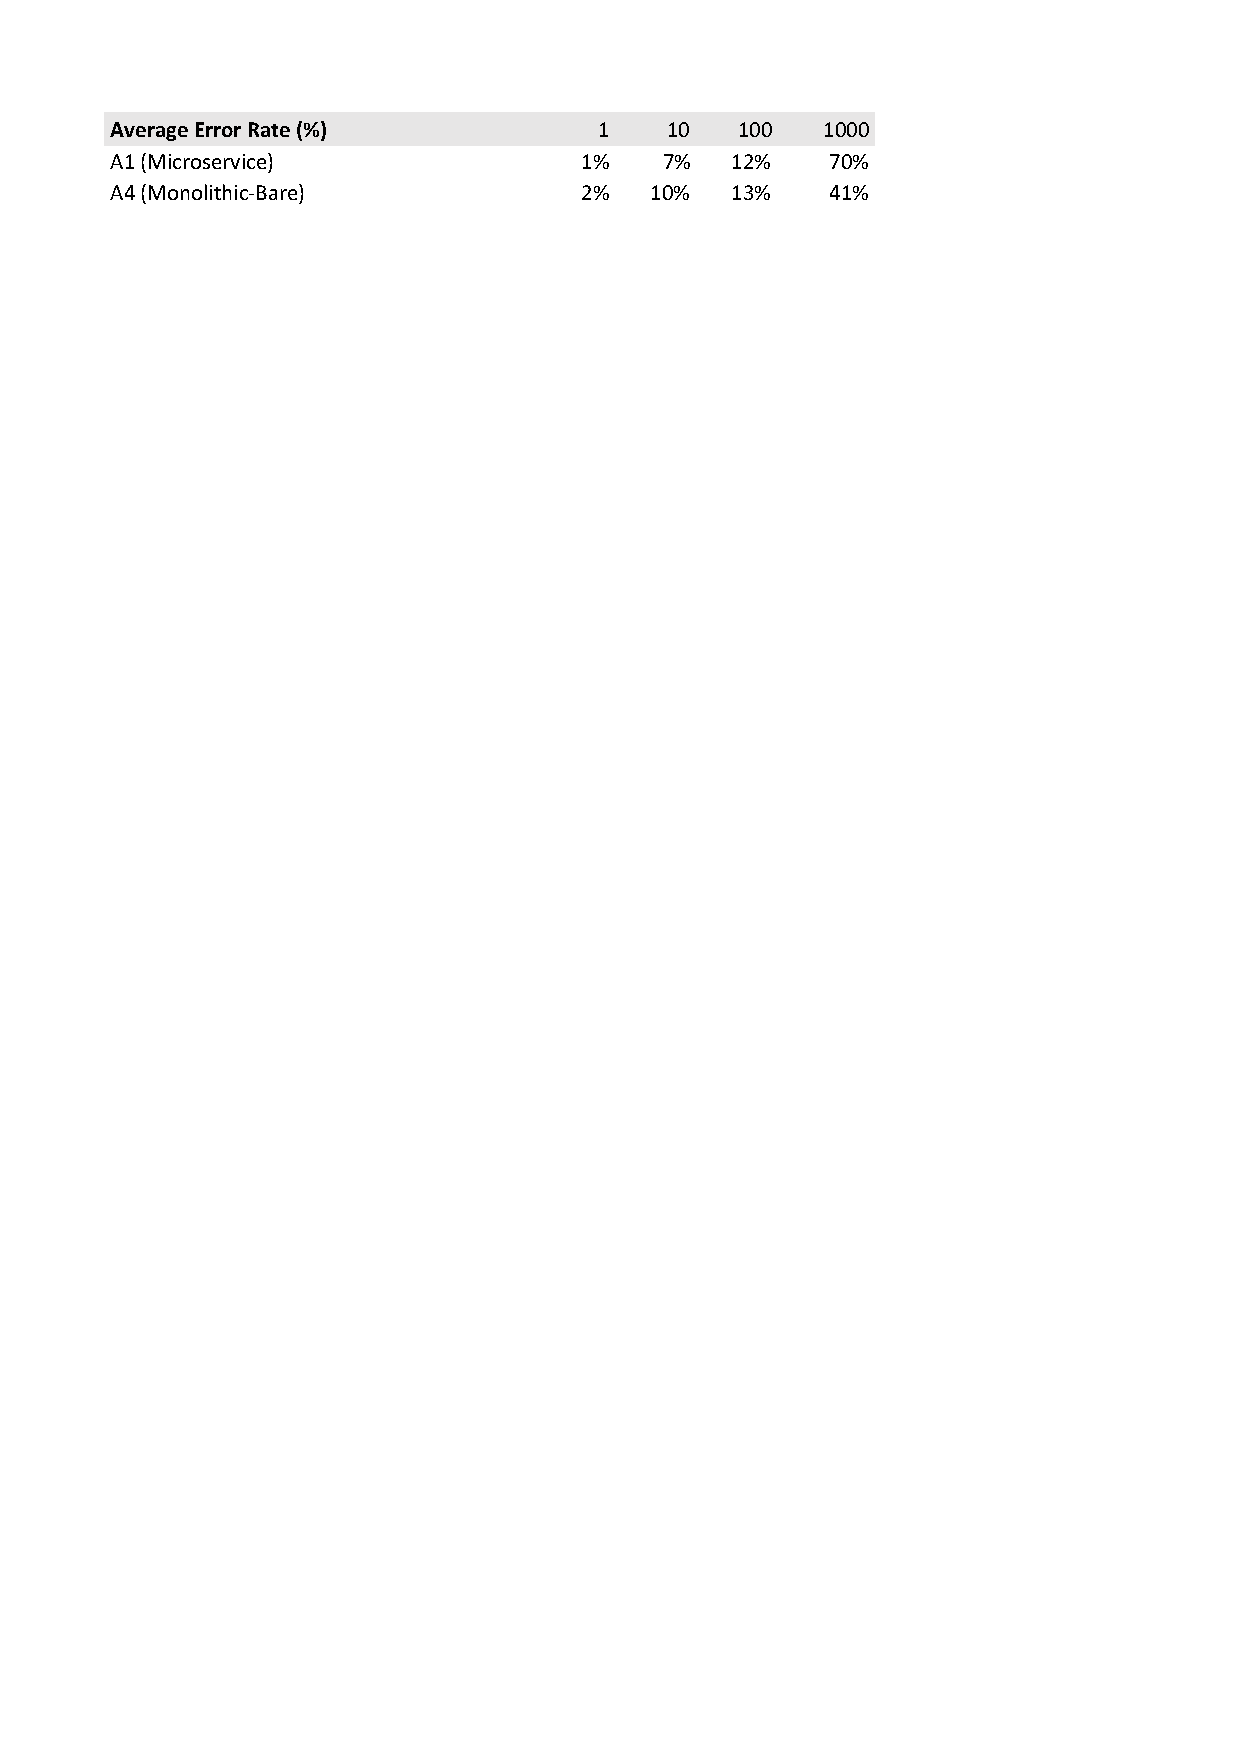
\includegraphics[trim={1cm 26cm 0 2cm},clip]{rq1-error}
\caption{Comparison table of the error rate in A1 and A4}
\label{rq1-error}
\end{center}
\end{figure}

%%%%%%%%%%%%%%%%%%%%%%%%%%%%%%%%%%%%%%%%%%%%%%%%%%%%%

\section{Containerized monolithic versus monolithic bare-metal (RQ2)}
%SHORT SUMMARY OF RQ AND THEN FOLLOW UP WITH EVERYTHING RELATED TO RQ
RQ2 aims to provide an answer about the performance difference when running an application in the A4 monolithic architecture compared to the A3 containerized (Docker) monolithic architecture.

\par\vspace{0.5cm}
When running our tests on the A3 containerized monolithic architecture we found that the average CPU usage was 44.37\% and the total memory usage was 7.47 GiB. When running our tests on the A4 monolithic architecture bare-metal we found that the average CPU usage was 49.12\% and the total memory usage was 8.07 GiB.

\par\vspace{0.5cm}
This means that we saw an increase of 4.75 percentage points in CPU usage in the bare-metal monolithic architecture using 0.6 GiB more RAM than the containerized application.

\par\vspace{0.5cm}
In figure \ref{rq2-latency}a and \ref{rq2-latency}b we can observe the difference in latency between A3 and A4. In this figure, we can see that A3 has lower or equal latency in all test cases.
For one user, we see that A3 is 7\% faster, for 10 users we can see that A3 is 9\% faster, for 100 users A3 is 9\% faster, and lastly for 1000 users A3 has the same latency as A4. 

\par\vspace{0.5cm}
Furthermore, we can see the throughput of successfully request in figure \ref{rq2-stps}. In this figure, we can see that A3 has higher or equal throughput in all test cases compared to A4. For one user, we can see that A3 has the same successful throughput as A4, for 10 users it has 5\% higher, for 100 users it has 8\% higher and for 1000 users it has 19\% higher successful throughput. 

\begin{figure}[h]
\begin{center}

\begin{subfigure}[b]{1\textwidth}
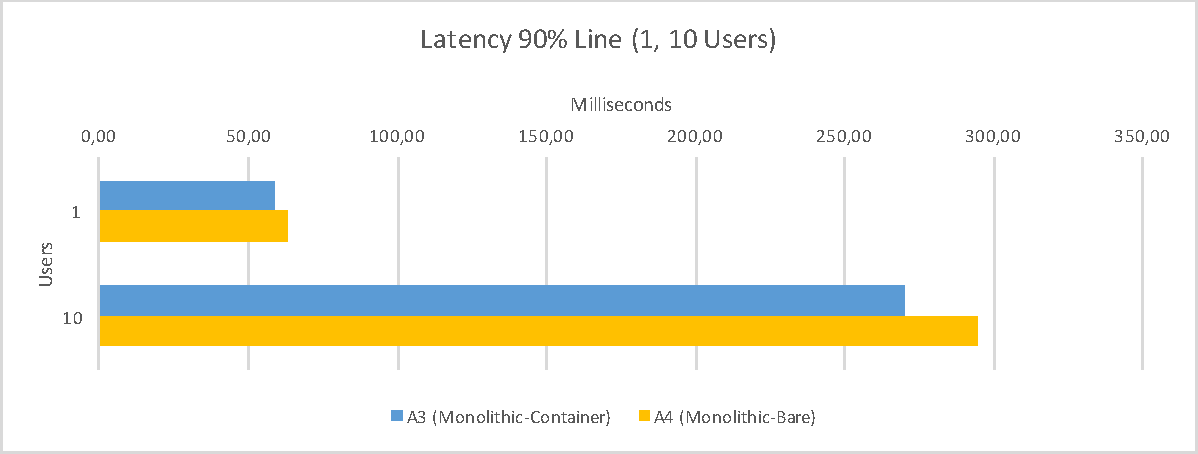
\includegraphics[width=13cm]{Graph/rq2-latency-1}
\caption{Comparison of the latency in A3 and A4 for 1 and 10 users}
\end{subfigure}

\begin{subfigure}[b]{1\textwidth}
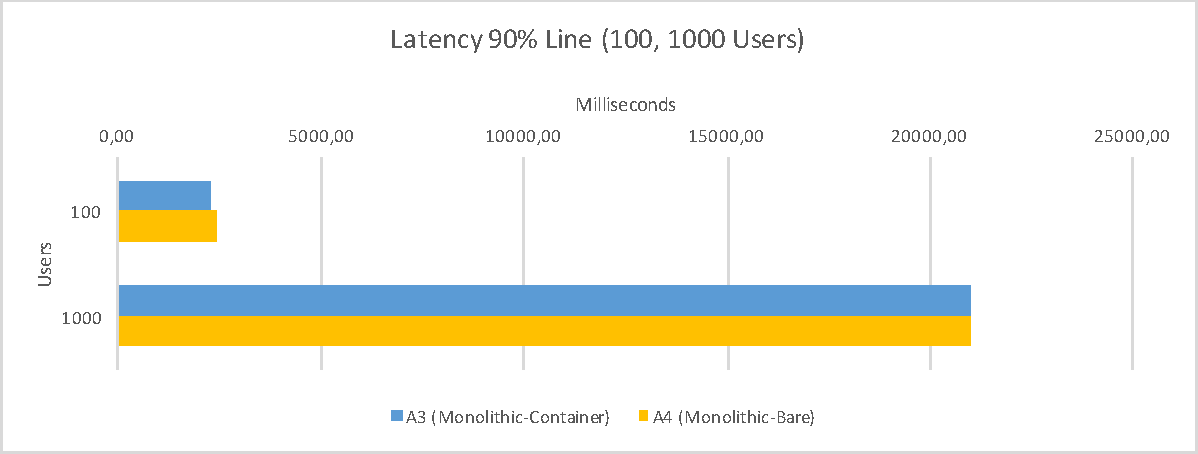
\includegraphics[width=13cm]{Graph/rq2-latency-2}
\caption{Comparison of the latency in A3 and A4 for 100 and 1000 users}
\end{subfigure}

\caption{Comparison of the latency in A3 and A4}
\label{rq2-latency}

\end{center}
\end{figure}


\begin{figure}[h]
\begin{center}

\begin{subfigure}[b]{1\textwidth}
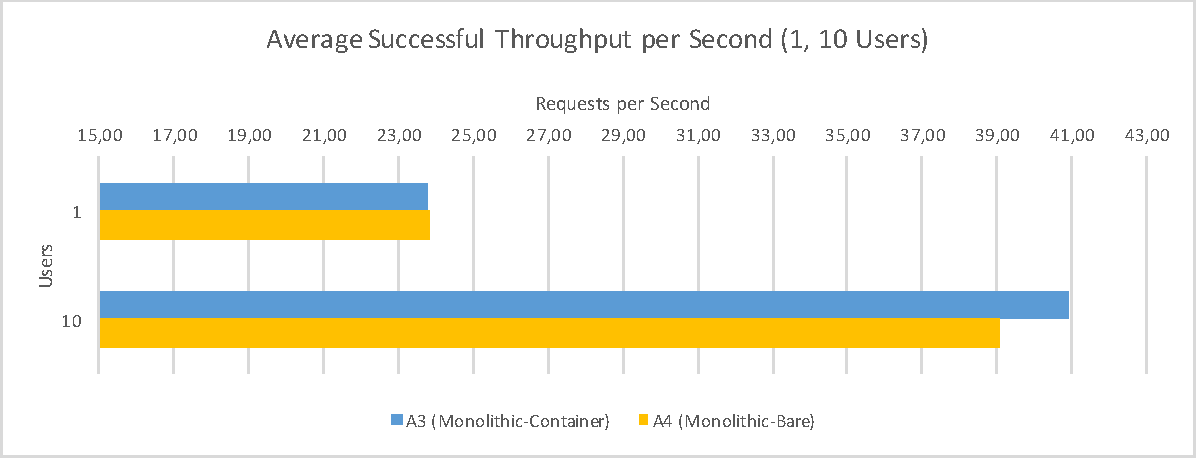
\includegraphics[width=13cm]{Graph/rq2-stps-1}
\caption{Comparison of the successful throughput in A3 and A4 for 1 and 10 users}
\end{subfigure}

\begin{subfigure}[b]{1\textwidth}
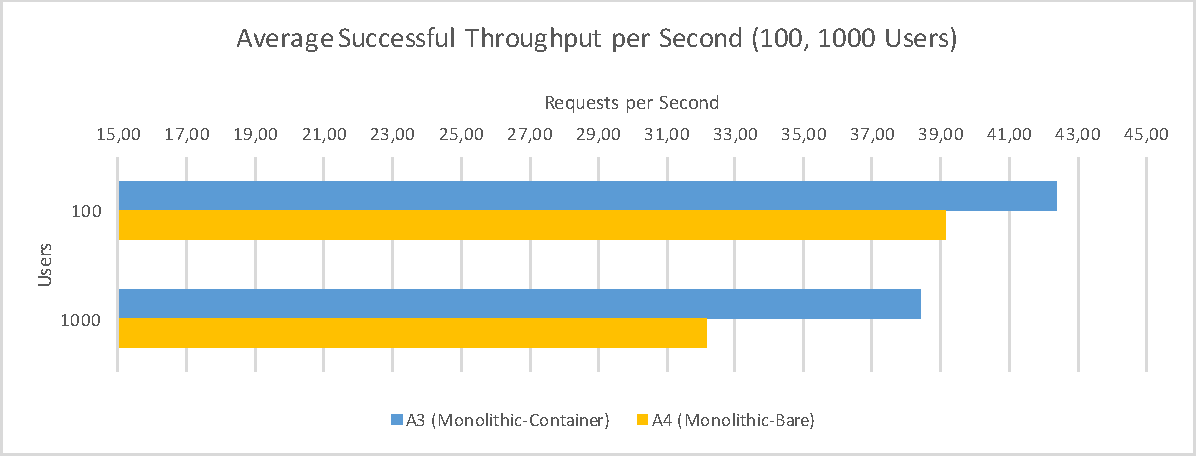
\includegraphics[width=13cm]{Graph/rq2-stps-2}
\caption{Comparison of the successful throughput in A3 and A4 for 100 and 1000 users}
\end{subfigure}

\caption{Comparison of the successful throughput inA3 and A4}
\label{rq2-stps}

\end{center}
\end{figure}

%%%%%%%%%%%%%%%%%%%%%%%%%%%%%%%%%%%%%%%%%%%%%%%%%%%%%

\section{Microservice on one machine versus a computer cluster (RQ3)}
%SHORT SUMMARY OF RQ AND THEN FOLLOW UP WITH EVERYTHING RELATED TO RQ
RQ3 aims to provide an answer about the performance difference when running an application in the A1 microservice architecture on one machine compared to running the A2 microservice architecture on several machines (computer cluster).

\par\vspace{0.5cm}
When running our tests on the A1 microservice architecture we found that the average CPU usage was 46.65\% and the total memory usage was 13.42 GiB.

\par\vspace {0.5cm}
When running our tests on the A2 cluster microservice architecture we found that the average CPU usage for the REST plus Cassandra computer was 5.86\% and the total memory usage was 7.83 GiB. For the computer running the microservices applications, the average CPU usage was 51.57\% and the total memory usage was 7.66 GiB RAM. This means we got a total RAM usage of 15.49 GiB with a higher CPU load on the computer running the microservices applications.

\par\vspace{0.5cm}
This means that the clustered used a total of 57\% CPU, 10.78 percentage points more than the non-clustered architecture. The clustered version also used 2.07 GiB RAM more than the non-clustered.

\par\vspace{0.5cm}
In figure \ref{rq3-latency}a and \ref{rq3-latency}b we can observe the difference in latency between A1 and A2. In this figure, we can see that A1 has lower latency in all test cases except the 100 users test case. For one user, we see that A1 is 15\% faster, for 10 users we can see that A1 is 2\% faster, for 100 users A1 is 2\% slower, and lastly for 1000 users A1 is 2\% faster than A2.

\par\vspace{0.5cm}
Furthermore, we can see the throughput of successfully request in figure \ref{rq3-stps}. In this figure, we can see that A2 has a higher throughput rate in all test cases except the 1 user test case. For one user, we can see that A1 has 13\% higher successful throughput than A2, for 10 users it has 4\% lower, for 100 users it has 7\% lower and for 1000 users it has 15\% lower successful throughput compared to A2.

\begin{figure}[h]
\begin{center}

\begin{subfigure}[b]{1\textwidth}
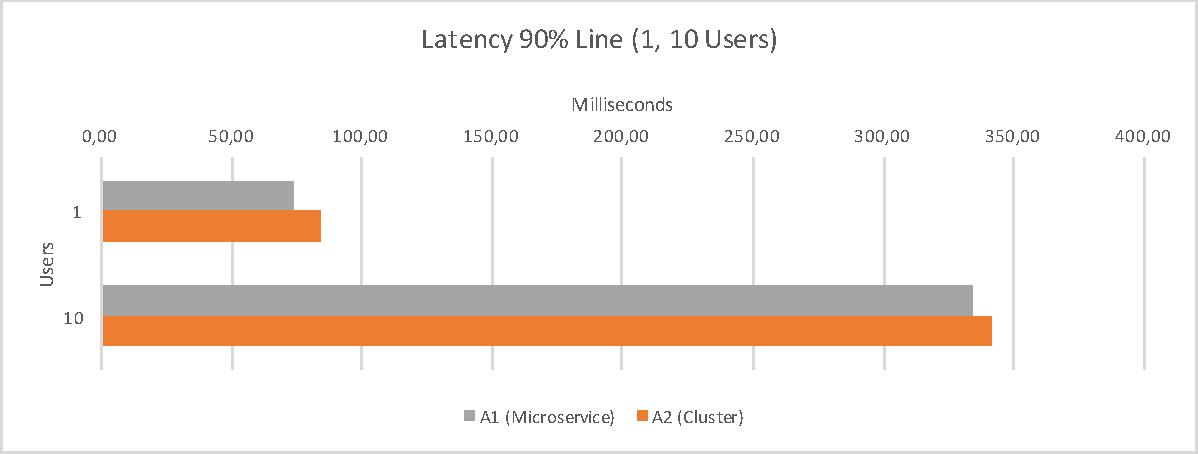
\includegraphics[width=12cm]{Graph/rq3-latency-1}
\caption{Comparison of the latency in A1 and A2 for 1 and 10 users}
\end{subfigure}

\begin{subfigure}[b]{1\textwidth}
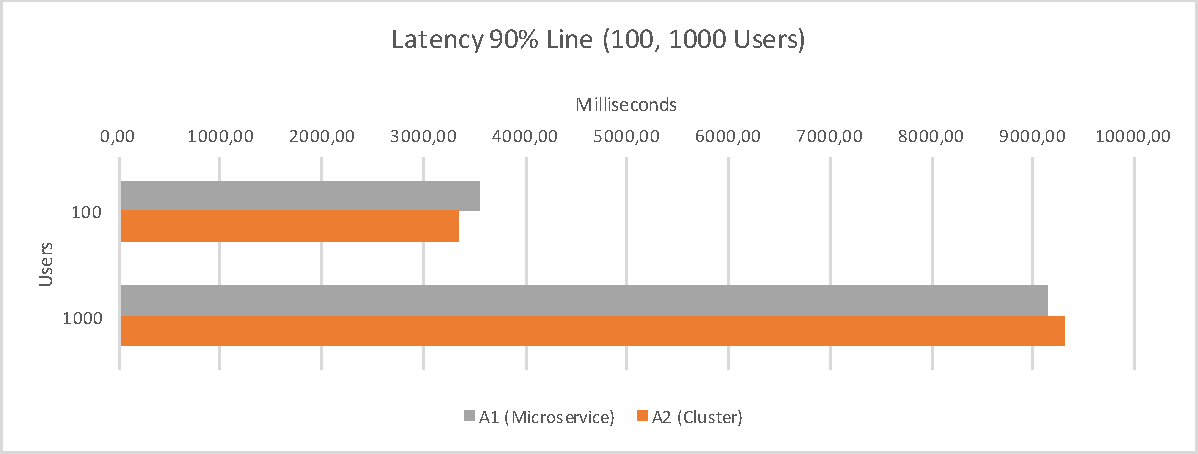
\includegraphics[width=12cm]{Graph/rq3-latency-2}
\caption{Comparison of the latency in A1 and A2 for 1 and 10 users}
\end{subfigure}

\caption{Comparison of the latency in A1 and A2}
\label{rq3-latency}

\end{center}
\end{figure}


\begin{figure}[h]
\begin{center}

\begin{subfigure}[b]{1\textwidth}
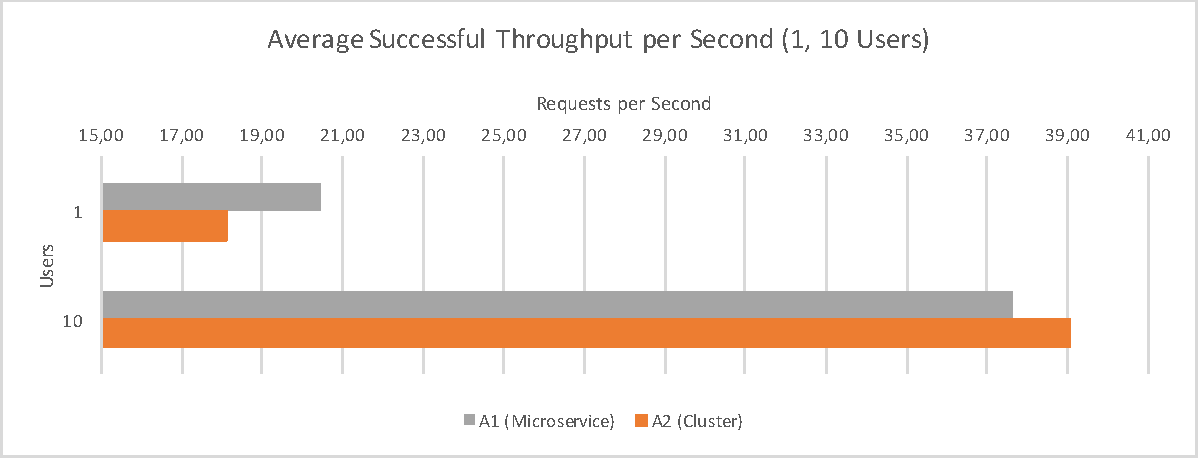
\includegraphics[width=13cm]{Graph/rq3-stps-1}
\caption{Comparison of the successful throughput in A1 and A2 for 1 and 10 users}
\end{subfigure}

\begin{subfigure}[b]{1\textwidth}
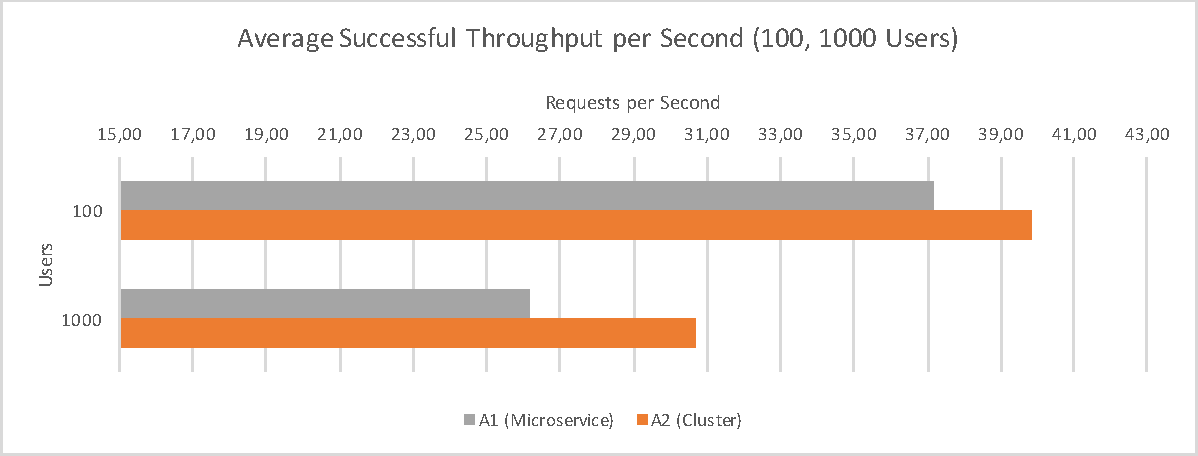
\includegraphics[width=13cm]{Graph/rq3-stps-2}
\caption{Comparison of the successful throughput in A1 and A2 for 100 and 1000 users}
\end{subfigure}


\caption{Comparison of the successful throughput in A1 and A2}
\label{rq3-stps}

\end{center}
\end{figure}


%%%%%%%%%%%%%%%%%%%%%%%%%%%%%%%%%%%%%%%%%%%%%%%%%%%%%

\clearpage
\par\vspace {0.5cm}

\chapter{Analysis} \label{Analysis}
%Always end your discussion with a summary that briefly recaps how your F has allowed you to answer the RQ and how this RQ is a contribution to the P and A that it is related to.
Our research aims to provide a more conclusive answer in the area of microservice architecture versus monolithic architecture where we focused on three questions explained previously in this thesis. In this chapter, we will go through each question one by one and present our result and compare it to previously made research.

% RQ1
\section{Monolithic architecture versus microservice architecture (RQ1)}
As shown in our Results we can see that the A4 monolithic bare-metal architecture will consume about a third of the memory, and nearly consume the same amount of CPU resources as the A1 microservice architecture with only 2.47 percentage points difference. This result show us that the A4 bare-metal monolithic architecture is more resource friendly with higher hardware efficiency compared to the A1 microservice architecture. 

\par\vspace{0.5cm}
Furthermore, we can see that the A4 bare-metal monolithic architecture has lower latency in figure \ref{rq1-latency}a and \ref{rq1-latency}b excluding the 1000 users test case because of the high error rate of the A1 microservice architecture that can be seen in figure \ref{rq1-error}. The high error rate is present because the system cannot handle the number of parallel users and therefore denies the request immediately.

\par\vspace{0.5cm}
Continuing looking at the successful throughput in figure \ref{rq1-stps}a and \ref{rq1-stps}b we once again can see that the A4 bare-metal monolithic architecture has higher performance than the A1 microservice architecture.

\par\vspace{0.5cm}
Important aspects of the results are that the A1 microservice architecture has up to 19\% lower successful throughput rate, and up to 31\% (excluding the 1000 users test case as explain before) slower response time than the A4 bare-metal monolithic architecture.

\par\vspace{0.5cm}
Our result is very similar to the result in Villamizar et al. paper \cite{Villamizar}, where this proves that microservices is slower in some extent but depends deeply on the number of concurrent users. Furthermore, this provides leverage for companies to evaluate if they should use the microservice architecture or not depending on their use case. Comparing our results to Ueda's paper there is a bigger difference in performance and monolithic is the big winner \cite{Ueda}. The reason for may be that the system they used an existing system which may be more suited for the monolithic architecture.
Finally, we believe that microservice architecture is here to stay with almost the same performance as the monolithic architectures and with the benefit scalability presented in Joy's article \cite{Joy}.

% RQ2
\section{Containerized monolithic versus bare-metal monolithic (RQ2)}
In our Results, we can see that the A3 containerized monolithic application uses 4.75 percentage points fewer CPU resources and 11\% less memory than the A4 monolithic bare-metal application.

\par\vspace{0.5cm}
Furthermore, we can see that the A3 containerized monolithic architecture have higher successful throughput and lower latency, even though it uses fewer computer resources. The A3 containerized monolithic application manages to get a higher successful throughput of up to 19\% where we also observed that the performance improvement seems to increase for every added concurrent user. However, in the case of latency, the difference seems pretty steady ranging from 0-9\% improvement over the A4 bare-metal monolithic application no matter what the number of users are.

\par\vspace{0.5cm}
These results are in line with Knoche \cite{Knoche} on the reasoning that the A3 containerized monolithic application have near the performance aspects of the A4 bare-metal monolithic application, and in some cases even higher performance, observed by Kalidindi \cite{Kalidindi}. In Kalidindi's study, there was a latency overhead of 6-8\% in Cassandra which was not seen in our case. This confirms that containerizing with Docker is not a bottleneck and this also proves that the decrease in performance of the microservices in RQ1 is not because of containerizing. 

% RQ3
\section{Microservice on one machine versus a computer cluster (RQ3)}
As shown in our Results we can see that the A2 computer cluster architecture have a marginally higher successful throughput compared to the A1 microservice architecture when having many concurrent users, but in terms of latency, the A1 microservice architecture responds faster in all test cases but one.

\par\vspace{0.5cm}
Furthermore, we can see that the A1 microservice architecture is utilizing the resources more efficiently with 10.78 percentage points less CPU and 15\% less RAM than the clustered version. The latency improvement in A1 ranges from 6\% slower in one case and up to 15\% improvement with only one concurrent user. The throughput for A1 is only more in the case of one user, for all the other test cases A2 is 4-15\% faster with a trend of the improvement increasing with more users.

\par\vspace{0.5cm}
We chose to compare the A2 computer cluster architecture with the A1 microservice architecture because of the reason that we wanted to see what the performance difference could be when the microservices where communicating between computers instead of only using Docker bridge. We have gotten a good insight of what the performance differences it brings and why it would not be too beneficial for running a cluster on a small-scale application with a low amount of users. But where we think that running a bigger computer cluster a local network can be beneficial with the correct architecture, with more efficiently used hardware.

%%%%%%%%%%%%%%%%%%%%%%%%%%%%%%%%%%%%%%%%%%%%%%%%%%%%%
\chapter{Conclusions and future work} \label{Conclusion}

This thesis set out to measure the performance differences in running a self-developed minimal microservice-based system and compare it with a monolithic counterpart. We measured the impact of running a system in container and lastly the difference in running a microservice cluster compared to microservices architecture on a single computer.\\

Through running a load testing tool called JMeter for simulating the users, we have found that a monolithic system has lower response times and higher throughput while using less RAM and CPU than a microservices system. We also found that using Docker to containerize a system does not decrease performance but in our case increased the performance on the aspect of RAM, CPU, successful throughput and latency.\\

The last thing we found was that when running the microservices architecture in a cluster compared to only using one computer, the latency was similar but throughput was increased by up to 15\% when the load on the system was high. The clustered version also used 15\% more RAM and about 11 percentage points more CPU.\\

These findings are important contributions to anyone looking over their architecture for the benefit of some aspects as modularity and scalability. Our findings provide both data and conclusions of when and where the microservice architecture could be beneficial over the monolithic architecture. While we have specifically focused on the performance between microservice architecture and monolithic architecture, we have also made contributions about Docker and running microservices in a computer cluster. These areas imply that our findings are likely to be of importance to anyone also looking at how Docker affects performance and how running microservice in a computer cluster affects performance. 

\par\vspace{0.5cm}
For future work, we would like to develop a more complex application with more parts and more complex functions and calculations as we believe features such as these will affect the performance of both monolithic and microservice-based applications.

\par\vspace{0.5cm}
We would like to extend our experiments in this research to other microservice architectures such as that each microservice has their own database. Another important topic that was not researched in this paper is the scalability of the microservice architecture compared to the monolithic architecture. We also think for orchestration of microservices need to be evaluated and how this affect the performance of a microservice application.

\bibliography{BibTeX}{}
\bibliographystyle{unsrt}

\end{document}
